\documentclass[12pt,a4paper]{article}

% 导入必要的宏包
\usepackage[UTF8]{ctex}
\usepackage{geometry}
\usepackage{amsmath}
\usepackage{amsfonts}
\usepackage{amssymb}
\usepackage{graphicx}
\usepackage{enumitem}
\usepackage{xcolor}
\usepackage{tikz}
\usepackage{float}
\usepackage{hyperref}
\usepackage{multicol}
\usepackage{longtable}
\usepackage{array}
\usepackage{tabularx}
\usepackage{listings}

% 代码高亮设置
\lstset{
    basicstyle=\ttfamily\small,
    keywordstyle=\color{blue},
    commentstyle=\color{green!70!black},
    stringstyle=\color{red},
    breaklines=true,
    numbers=left,
    numberstyle=\tiny\color{gray},
}

% 页面设置
\geometry{left=2.5cm,right=2.5cm,top=2.5cm,bottom=2.5cm}

% 标题页设置
\title{\textbf{2013年数据结构题库} \\ \large 单项选择题与综合应用题详解}
\author{}
\date{}

% 定义题型环境
\newenvironment{choicequestion}[1][]{%
    \vspace{0.5cm}
    \noindent\textbf{[#1]}
    \vspace{0.2cm}
}{}

\newenvironment{answersection}{%
    \vspace{0.2cm}
    \noindent\textbf{[参考答案]}\\
    \vspace{0.1cm}
}{}

\newenvironment{analysissection}{%
    \vspace{0.2cm}
    \noindent\textbf{[答案解析]}\\
    \vspace{0.1cm}
}{}

% 定义题号计数器
\newcounter{questioncounter}

% 定义题号计数器
\newcounter{questioncounter}

% 问题格式化命令
\newcommand{\question}[2]{%
    \stepcounter{questioncounter}%
    \noindent\textbf{\thequestioncounter} #1%
}

% 选择题选项格式
\newcommand{\choices}[4]{%
    \begin{multicols}
    \noindent \textbf{A.} #1 \par
    \noindent \textbf{B.} #2 \par
    \noindent \textbf{C.} #3 \par
    \noindent \textbf{D.} #4 \par
    \end{multicols}%
}

% 开始文档
\begin{document}

\maketitle

\section{单项选择题}

\begin{choicequestion}[单选题]
\question{已知两个长度分别为 $m$ 和 $n$ 的升序链表，若将它们合并为一个长度为 $m + n$ 的降序链表，则最坏情况下的时间复杂度是}{}

\choices{$\mathrm{O}(n)$}{$\mathrm{O}(mn)$}{$\mathrm{O}(\min(m,n))$}{$\mathrm{O}(\max(m,n))$}

\begin{answersection}
D. $\mathrm{O}(\max(m,n))$
\end{answersection}

\begin{analysissection}
要将两个升序链表合并为降序链表，可先将两个链表反转（或从尾部比较），然后按降序合并。无论哪种方式，最坏情况下均需遍历两个链表的所有结点，总时间复杂度为 $O(m+n)$，即 $O(\max(m,n))$。
\end{analysissection}
\end{choicequestion}

\begin{choicequestion}[单选题]
\question{一个栈的入栈序列为 $1, 2, 3, \dots, n$ ，其出栈序列是 $\mathfrak{p}_1, \mathfrak{p}_2, \mathfrak{p}_3, \dots, \mathfrak{p}_n$ 。若 $\mathfrak{p}_2 = 3$ ，则 $\mathfrak{p}_3$ 可能取值的个数是}{}

\choices{$n - 3$}{$n - 2$}{$n - 1$}{无法确定}

\begin{answersection}
C. $n - 1$
\end{answersection}

\begin{analysissection}
$p_2=3$ 表明在3出栈前，1和2已入栈，且3入栈后立即出栈。此时栈中至少有1、2（栈顶为2），后续可出栈的元素包括2、1，以及后续入栈的4至n。因此$p_3$可取2、1或4至n，共$n-1$种可能值。
\end{analysissection}
\end{choicequestion}

\begin{choicequestion}[单选题]
\question{若将关键字 1,2,3,4,5,6,7 依次插入到初始为空的平衡二叉树 T 中，则 T 中平衡因子为 0 的分支结点的个数是}{}

\choices{0}{1}{2}{3}

\begin{answersection}
B. 1
\end{answersection}

\begin{analysissection}
依次插入1~7后，树需多次旋转以保持平衡。最终形成的平衡二叉树中，仅根结点（通常为4）的平衡因子为0，其余分支结点平衡因子为±1。
\end{analysissection}
\end{choicequestion}

\begin{choicequestion}[单选题]
\question{已知三叉树 T 中 6 个叶结点的权分别是 2,3,4,5,6,7，T 的带权（外部）路径长度最小是}{}

\choices{27}{46}{54}{56}

\begin{answersection}
B. 46
\end{answersection}

\begin{analysissection}
构造带权三叉哈夫曼树（每次合并三个最小权值结点）。叶子权值2,3,4,5,6,7（6个为偶数，需添加权值为0的虚拟结点）。经合并后，最小带权路径长度WPL=46。
\end{analysissection}
\end{choicequestion}

\begin{choicequestion}[单选题]
\question{若 X 是后序线索二叉树中的叶结点，且 X 存在左兄弟结点 Y，则 X 的右线索指向的是}{}

\choices{X 的父结点}{以 $\mathrm{Y}$ 为根的子树的最左下结点}{X 的左兄弟结点 Y}{以 $\mathrm{Y}$ 为根的子树的最右下结点}

\begin{answersection}
A. X 的父结点
\end{answersection}

\begin{analysissection}
后序遍历顺序为“左-右-根”。叶结点X有左兄弟Y时，在后序序列中X之后紧接其父结点（X是父结点右子树中最后访问的结点）。因此X的右线索指向其父结点。
\end{analysissection}
\end{choicequestion}

\begin{choicequestion}[单选题]
\question{在任意一棵非空二叉排序树 $\mathrm{T}_{1}$ 中，删除某结点 $\mathbf{v}$ 之后形成二叉排序树 $\mathrm{T}_{2}$ ，再将 $\mathbf{v}$ 插入 $\mathrm{T}_{2}$ 形成二叉排序树 $\mathrm{T}_{3}$ 。下列关于 $\mathrm{T}_{1}$ 与 $\mathrm{T}_{3}$ 的叙述中，正确的是\newline
I. 若 $\mathbf{v}$ 是 $\mathrm{T}_{1}$ 的叶结点，则 $\mathrm{T}_{1}$ 与 $\mathrm{T}_{3}$ 不同\newline
II. 若 $\mathbf{v}$ 是 $\mathrm{T}_{1}$ 的叶结点，则 $\mathrm{T}_{1}$ 与 $\mathrm{T}_{3}$ 相同\newline
III. 若 $\mathrm{v}$ 不是 ${\mathrm{T}}_{1}$ 的叶结点,则 ${\mathrm{T}}_{1}$ 与 ${\mathrm{T}}_{3}$ 不同\newline
IV. 若 $\mathrm{v}$ 不是 ${\mathrm{T}}_{1}$ 的叶结点,则 ${\mathrm{T}}_{1}$ 与 ${\mathrm{T}}_{3}$ 相同}{}

\choices{仅 I、III}{仅 I、IV}{仅 II、III}{仅 II、IV}

\begin{answersection}
C. 仅 II、III
\end{answersection}

\begin{analysissection}
- 若v是叶结点，删除后插入原位置，T1=T3（II正确，I错误）；
- 若v是非叶结点，删除时用前驱或后继替代，插入后位置改变，T1≠T3（III正确，IV错误）。

故正确的是II和III。
\end{analysissection}
\end{choicequestion}

\begin{choicequestion}[单选题]
\question{设图的邻接矩阵 $A$ 如下所示。各顶点的度依次是
$$
A = \left[ \begin{array}{cccc} 
0 & 1 & 0 & 1 \\ 
0 & 0 & 1 & 1 \\ 
0 & 1 & 0 & 0 \\ 
1 & 0 & 0 & 0 
\end{array} \right]
$$}{}

\choices{1,2,1,2}{2,2,1,1}{3,4,2,3}{4, 4, 2, 2}

\begin{answersection}
C. $3,4,2,3$
\end{answersection}

\begin{analysissection}
该矩阵为有向图邻接矩阵，顶点度数为入度+出度：
- 顶点0：出度2，入度1 → 度3
- 顶点1：出度2，入度2 → 度4
- 顶点2：出度1，入度1 → 度2
- 顶点3：出度1，入度2 → 度3

各顶点度数依次为3,4,2,3。
\end{analysissection}
\end{choicequestion}

\begin{choicequestion}[单选题]
\question{若对如下无向图进行遍历，则下列选项中，不是广度优先遍历序列的是}{}

\begin{figure}[H]
\centering
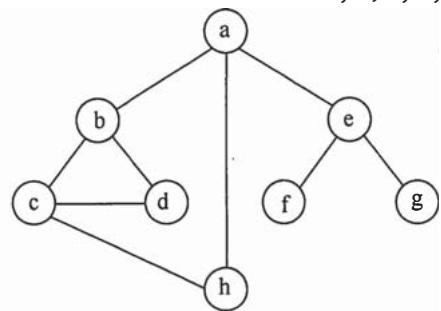
\includegraphics[width=0.4\textwidth]{images/eeff0cc1739b47836885102e4a27a7118d37dfd488c1106ba8dd7d020fdf3464.jpg}
\end{figure}

\choices{h, c, a, b, d, e, g, f}{e, a, f, g, b, h, c, d}{d, b, c, a, h, e, f, g}{a, b, c, d, h, e, f, g}

\begin{answersection}
D. a, b, c, d, h, e, f, g
\end{answersection}

\begin{analysissection}
BFS按层次依次访问邻接结点。选项D中从a访问b、c后直接跳到d、h，违背层次访问顺序，不可能是BFS序列。其余序列均可能通过不同起始点或邻接顺序得到。
\end{analysissection}
\end{choicequestion}

\begin{choicequestion}[单选题]
\question{下列 AOE 网表示一项包含 8 个活动的工程。通过同时加快若干活动的进度可以缩短整个工程的工期。下列选项中, 加快其进度就可以缩短工程工期的是}{}

\begin{figure}[H]
\centering
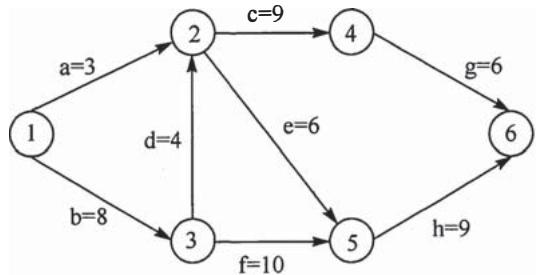
\includegraphics[width=0.4\textwidth]{images/ad83808691bd14cd04fe9d1fcd61f2f3c684f4df4f9e04a8f612a714678243e4.jpg}
\end{figure}

\choices{c 和 e}{d 和 e}{f和d}{f和h}

\begin{answersection}
A. c 和 e
\end{answersection}

\begin{analysissection}
AOE网中关键路径上的活动为关键活动，缩短其持续时间可缩短总工期。图中c和e位于关键路径上，故加快二者进度可缩短工期。
\end{analysissection}
\end{choicequestion}

\begin{choicequestion}[单选题]
\question{在一棵高度为 2 的 5 阶 B 树中，所含关键字的个数最少是}{}

\choices{5}{7}{8}{14}

\begin{answersection}
A. 5
\end{answersection}

\begin{analysissection}
5阶B树中非根结点至少含2个关键字，根结点至少含1个关键字。高度为2的最小B树：根含1个关键字，2个子结点各含2个关键字，总关键字数=1+2×2=5。
\end{analysissection}
\end{choicequestion}

\begin{choicequestion}[单选题]
\question{对给定的关键字序列110,119,007,911,114,120,122进行基数排序，则第2趟分配收集后得到的关键字序列是}{}

\choices{007, 110, 119, 114, 911, 120, 122}{007, 110, 119, 114, 911, 122, 120}{007, 110, 911, 114, 119, 120, 122}{110, 120, 911, 122, 114, 007, 119}

\begin{answersection}
A. 007, 110, 119, 114, 911, 120, 122
\end{answersection}

\begin{analysissection}
基数排序从低位到高位。第1趟按个位排序后序列为110,120,122,114,007,119,911；第2趟按十位排序后得到007,110,114,119,911,120,122（对应选项A）。
\end{analysissection}
\end{choicequestion}

\section{综合应用题}

\begin{choicequestion}[问答题]
\question{（13分）已知一个整数序列 $\mathrm{A} = (a_{0}, a_{1}, \dots, a_{n - 1})$ ，其中 $0 \leqslant a_{i} < n$ （ $0 \leqslant i < n$ ）。若存在 $a_{p1} = a_{p2} = \dots = a_{pm} = x$ 且 $m > n / 2$ （ $0 \leqslant p_{k} < n, 1 \leqslant k \leqslant m$ ），则称 $x$ 为 A 的主元素。试设计一个尽可能高效的算法，找出 A 的主元素。若存在主元素，则输出该元素；否则输出-1。要求：\newline
(1) 给出算法的基本设计思想。  \newline
(2) 根据设计思想, 采用 C 或 C++ 语言描述算法, 关键之处给出注释。  \newline
(3) 说明你所设计算法的时间复杂度和空间复杂度。}{}

\begin{answersection}
(1) 算法的基本设计思想：采用Boyer-Moore多数投票算法。先通过一次遍历找出候选主元素，再通过第二次遍历验证其出现次数是否超过$n/2$。
\end{answersection}

\begin{analysissection}
(2) C语言实现：
\begin{lstlisting}[language=C]
int majorityElement(int A[], int n) {
    int candidate = -1, count = 0;
    for (int i = 0; i < n; i++) {          // 第一趟：找候选元素
        if (count == 0) {
            candidate = A[i];
            count = 1;
        } else if (A[i] == candidate) {
            count++;
        } else {
            count--;
        }
    }
    
    count = 0;
    for (int i = 0; i < n; i++) {          // 第二趟：验证
        if (A[i] == candidate) count++;
    }
    
    return (count > n / 2) ? candidate : -1;
}
\end{lstlisting}

(3) 时间复杂度：$O(n)$（两次线性遍历）；空间复杂度：$O(1)$（仅使用常数额外变量）。
\end{analysissection}
\end{choicequestion}

\begin{choicequestion}[问答题]
\question{（10分）设包含4个数据元素的集合 $\mathrm{S} = \{\text{"do"，"for"，"repeat"，"while"}\}$ ，各元素的查找概率依次为 $p_1 = 0.35$ ， $p_2 = 0.15$ ， $p_3 = 0.15$ ， $p_4 = 0.35$ 。将S保存在一个长度为4的顺序表中，采用折半查找法，查找成功时的平均查找长度为2.2。请回答：\newline
（1）若采用顺序存储结构保存S，且要求平均查找长度更短，则元素应如何排列？应使用何种查找方法？查找成功时的平均查找长度是多少？  \newline
(2) 若采用链式存储结构保存 S, 且要求平均查找长度更短, 则元素应如何排列? 应使用何种查找方法? 查找成功时的平均查找长度是多少?}{}

\begin{answersection}
(1) 顺序存储时，按查找概率从大到小排列元素（"do","while","for","repeat"或"while","do","for","repeat"），采用顺序查找，平均查找长度ASL=2.1。

(2) 链式存储时，按查找概率从大到小排列元素（头结点后接"do","while","for","repeat"），采用顺序查找，平均查找长度ASL=2.1。
\end{answersection}

\begin{analysissection}
按概率从大到小排列可最小化平均查找长度。对于顺序查找，ASL = $\sum i \cdot p_i$ = 1×0.35 + 2×0.35 + 3×0.15 + 4×0.15 = 2.1，比折半查找的2.2更优。
\end{analysissection}
\end{choicequestion}

\end{document}